\documentclass[a4paper,12pt,obeyspaces,spaces,hyphens]{article}

\usepackage{agenda}
\usepackage{colortbl}
\usepackage{xcolor}
\usepackage{palatino}
\usepackage{calc}

\hypersetup{pdftitle={Android System Development Training},
  pdfauthor={Free Electrons}}

\renewcommand{\arraystretch}{2.0}

\begin{document}

\thispagestyle{fancy}

\setlength{\arrayrulewidth}{0.8pt}

\begin{center}
\LARGE
Android System Development Training\\
\large
4-day session
\end{center}
\vspace{1cm}

\small
\newcolumntype{g}{>{\columncolor{fedarkblue}}m{4cm}}
\newcolumntype{h}{>{\columncolor{felightblue}}X}

\arrayrulecolor{lightgray} {
  \setlist[1]{itemsep=-5pt}
  \begin{tabularx}{\textwidth}{|g|h|}
    {\bf Title} & {\bf Android System Development Training}\\
    \hline

    {\bf Overview} &
    Understanding the Android Internals \par
    Understanding the Android Build System \par
    Customizing Android for a specific hardware \par
    Extending the Android framework \par
    Practical labs with the ARM-based BeagleBone Black board. \\
    \hline
    {\bf Materials} &
    Check that the course contents correspond to your needs:
    \url{http://free-electrons.com/doc/training/android} \\
    \hline

    {\bf Duration} & {\bf Four} days - 32 hours (8 hours per day).
    \newline 50\% of lectures, 50\% of practical labs. \\
    \hline

    {\bf Trainer} & One of the engineers listed on
    \newline \url{http://free-electrons.com/training/trainers/}\\
    \hline

    {\bf Language} & Oral lectures: English or French.
    \newline Materials: English.\\
    \hline

    {\bf Audience} & Engineers porting Android to new boards
    \newline Engineers developing products with Android \\
    \hline

    {\bf Prerequisites} & {\bf Knowledge and practice of Unix or
      GNU/Linux commands}
    \newline People lacking experience on this topic should get
    trained by themselves, for example with our freely available
    on-line slides:
    \newline \url{http://free-electrons.com/docs/command-line/} \vspace{1em}
    \newline {\bf Basics of Java programming} \\
    \hline
  \end{tabularx}

  \begin{tabularx}{\textwidth}{|g|h|}
    {\bf Required equipment} &
    {\bf For on-site sessions only}
    \newline Everything is supplied by Free Electrons in public sessions.
    \begin{itemize}
    \item Video projector
    \item PC computers with at least 4 GB of RAM, a CPU at least
      equivalent to an Intel Core i5 and Ubuntu Linux installed in a
      {\bf free partition of at least 60 GB. Using Linux in a virtual
        machine is not supported}, because of issues connecting to
      real hardware.
    \item We need Ubuntu Desktop 12.04 (64 bit, Xubuntu and Kubuntu
      variants are fine). We don't support other distributions,
      because we can't test all possible package versions.
    \item {\bf High Speed Connection to the Internet} (direct or
      through the company proxy), fast enough to download the several
      gigabytes of Android source code.
    \item {\bf PC computers with valuable data must be backed up}
      before being used in our sessions. Some people have already made
      mistakes during our sessions and damaged work data.
    \end{itemize} \\
    \hline

    {\bf Materials} & Print and electronic copies of presentations and
    labs.
    \newline Electronic copy of lab files.\\
    \hline

\end{tabularx}}
\normalsize

\feagendatwocolumn
{Hardware}
{
  The hardware platform used for the practical labs of this training
  session is the {\bf BeagleBone Black board}, which features:

  \begin{itemize}
  \item An ARM AM335x processor from Texas Instruments (Cortex-A8
    based), 3D acceleration, etc.
  \item 512 MB of RAM
  \item 2 GB of on-board eMMC storage
        \newline(4 GB in Rev C)
  \item USB host and device
  \item HDMI output
  \item 2 x 46 pins headers, to access UARTs, SPI buses, I2C buses
    and more.
  \end{itemize}
}
{}
{
  \begin{center}
    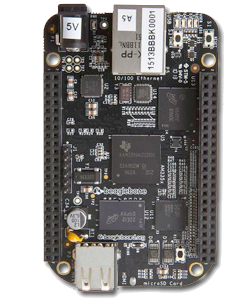
\includegraphics[height=5cm]{../slides/beagleboneblack-board/beagleboneblack.png}
  \end{center}
}

\section{Part 1 - Compiling and booting Android}

\feagendatwocolumn
{Lecture - Introduction to Android}
{
  \begin{itemize}
  \item History
  \item Actors involved
  \item Introduction to the Android architecture
  \end{itemize}
}
{Lab - Setup}
{
  \begin{itemize}
  \item Install the tools required to compile
  \item Fetch the source code (\textit{If the network bandwidth is not
      sufficient, we will provide a ready-to-use source code archive})
  \item Get used to Android specific tools
  \end{itemize}
}

\feagendatwocolumn
{Lecture - Android Source Code and Compilation}
{
  \begin{itemize}
  \item How to use git, repo and gerrit to access sources
  \item How to find one's way in the code base
  \item How to compile Android (tools, targets, etc.)
  \end{itemize}
}
{Lab - First Compilation}
{
  {\em Using the Android Emulator}
  \begin{itemize}
  \item Compile a first root filesystem for the emulator
  \end{itemize}
}

\feagendatwocolumn
{Lecture - Introduction to the Linux kernel}
{
  \begin{itemize}
  \item Role and general architecture of the kernel
  \item Kernel features
  \item Understanding the development process.
  \item Legal constraints with device drivers.
  \item Kernel user interface (/proc and /sys)
  \item Kernel configuration.
  \item Native and cross-compilation. Generated files.
  \end{itemize}
}
{Lab - Compile and Boot an Android Kernel}
{
  {\em Using the Android Emulator}
  \begin{itemize}
  \item Compile and Boot an Android Kernel
  \item Extract the patches from the Android Kernel
  \end{itemize}
}
\\
\section{Part 2 - Porting Android to a New Board}

\feagendaonecolumn
{Lecture - Changes introduced in the Android Kernel}
{
  \begin{itemize}
  \item Major functional changes introduced by Google
  \item Additions to the kernel
  \item Mainline kernel status of these patches
  \end{itemize}
}

\feagendatwocolumn
{Lecture - Android Bootloaders}
{
  \begin{itemize}
  \item What is a bootloader
  \item Bootloader examples
  \item The fastboot specifications from Android.
  \end{itemize}
}
{Lab - Supporting a board}
{
  {\em Using the BeagleBone Black board}
  \begin{itemize}
  \item Use the Android's build for the BeagleBone Black
  \item Boot Android on a real board
  \item Troubleshoot the glitches on the board
  \end{itemize}
}

\section{Part 3 - Device Development with Android}

\feagendatwocolumn
{Lecture – Developing and debugging with ADB}
{
  \begin{itemize}
  \item Presentation of ADB
  \item Available commands: transfer files,
    install packages, executing remote commands, log access,
    networking... all this done from the development machine.
  \item Examples of commands and combinations useful to debug
  \end{itemize}
}
{Lab – Use ADB}
{
  \begin{itemize}
  \item Learn how to get the system log, to gain access to a shell on
    the device, push and pull files, etc.
  \end{itemize}
}

\feagendaonecolumn
{Lecture – Android filesystem layout}
{
  \begin{itemize}
  \item Know where the various software components are installed and
    mounted, and why it matters.
  \end{itemize}
}

\feagendatwocolumn
{Lecture – Android build system}
{
  \begin{itemize}
  \item Concepts introduced in the build system
  \item Architecture of the Makefiles
  \item Variables and functions available
  \item Compilation steps
  \item Add a new device to the build system
  \end{itemize}
}
{Lab – Add a native library to the build}
{
  \begin{itemize}
  \item Create an external library to control a USB rocket launcher.
  \item Add this library to the default Android build
  \end{itemize}
}

\feagendaonecolumn
{Lab - System customization}
{
  \begin{itemize}
  \item Add a device to the build system
  \item Customize the “About” info, build ID, boot and home screens in
    your system.
  \end{itemize}
}

\feagendatwocolumn
{Lecture – Android Native Layer}
{
  \begin{itemize}
  \item Discover the daemons handling the radio, external storage,
    launching applications, etc.
  \item Get to know the different components involved in the Android
    runtime, from the virtual machine to the media framework:
    StageFright, Flingers, Dalvik...
  \item Learn how hardware abstraction is done in Android
  \end{itemize}
}
{Lab – Add a native binary to the build}
{
  \begin{itemize}
  \item Get to know the build system and the C library (Bionic)
    specifics.
  \end{itemize}
}

\feagendatwocolumn
{Lecture – Android Framework and Applications}
{
  \begin{itemize}
  \item Overview of the services, Content Providers and available
    applications in a standard Android build
  \item Structure of a Service / Content Provider
  \item How to access a native library from a Java app
    using the Java Native Interface (JNI)
  \end{itemize}
}
{Lab – Develop the Java interface to the native library}
{
  \begin{itemize}
  \item Implement a Java interface to use the previously integrated
    library
  \end{itemize}
}

\feagendatwocolumn
{Lecture – Android Application Development}
{
  \begin{itemize}
  \item The application lifecycle
  \item The various application components
  \item How to access services
  \item How to use, access and manage the resources
  \item How apk packages are built and what do they contain
  \end{itemize}
}
{Lab – Write an app with the SDK}
{
  \begin{itemize}
  \item Learn how to write and distribute an application using the
    Android SDK and its API.
  \item Practical case: write an Android application controlling the
    USB rocket launcher.
  \end{itemize}
}

\end{document}
